%% bulk_genome_comparisons.tex
%% Author: Leighton Pritchard
%% Copyright: James Hutton Institute
%% Bulk genome property comparisons

%
\begin{frame}
  \frametitle{Bulk property comparisons}
  \Large{
    \textcolor{olive}{
      \textbf{
      You don't have to sequence genomes to compare them \\
      (but it helps) \\
      }
    }
  }
\end{frame}

%
\begin{frame}
  \frametitle{Genome comparisons predate NGS}
  \begin{itemize}
    \item Sequence data wasn't always cheap and abundant
    \item Practical, experimental genome comparisons were needed
  \end{itemize}
  \begin{center}
    
\includegraphics[width=0.7\textwidth]{images/land_before_time}
  \end{center}  
\end{frame}

%
\begin{frame}
  \frametitle{Bulk property comparisons}
  \Large{
    \textcolor{olive}{
      \textbf{
      Calculate values for individual genomes, \\
      then compare them.
      }
    }
  }
  \normalsize{
        \begin{itemize}
         \item \textcolor{hutton_green}{Number of chromosomes}
         \item \textcolor{hutton_blue}{Ploidy}
         \item \textcolor{RawSienna}{Chromosome size}
         \item \textcolor{hutton_purple}{Nucleotide (A,C,G,T) frequency}        
        \end{itemize}
  }
\end{frame}

%
\begin{frame}
  \frametitle{Nucleotide frequency/genome size}
  Very easy to calculate from complete or draft genome sequence \\
  \begin{center}
    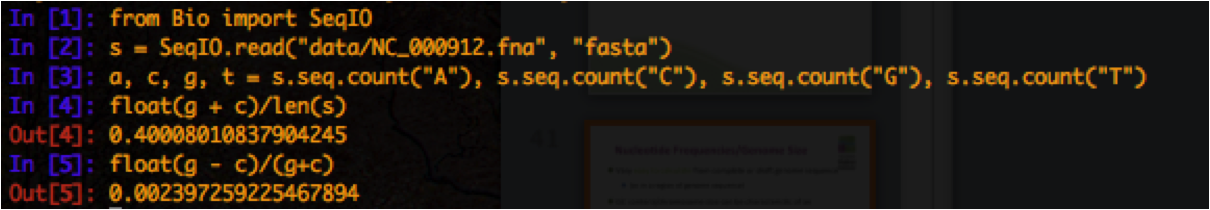
\includegraphics[width=\textwidth]{images/python_gc} \\
  \end{center}  
  GC content, chromosome size can be characteristic of an organism.
\end{frame}

%
\begin{frame}
  \frametitle{Genome Size and GC\%}
  \begin{center}
    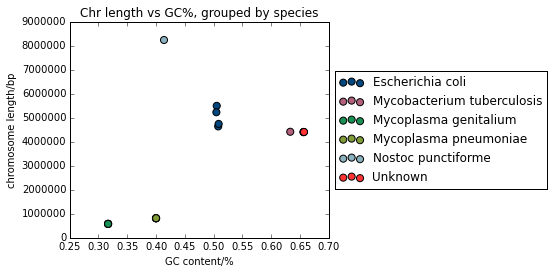
\includegraphics[width=\textwidth]{images/bacteria_gc_size}
  \end{center}
\end{frame}

%
\begin{frame}
  \frametitle{Blobology
  \footnote{\tiny{\href{http://dx.doi.org/10.1007/s13199-012-0154-6
}{Kumar \& Blaxter (2011) \textit{Symbiosis} doi:10.1007/s13199-012-0154-6
}}}
  \footnote{\tiny{\href{http://nematodes.org/bioinformatics/blobology/
}{http://nematodes.org/bioinformatics/blobology/
}}}  
  }
  Sequence data can be contaminated by other organisms
  \begin{itemize}
    \item \textcolor{hutton_green}{Host and symbiont DNA have different \%GC}
    \item \textcolor{hutton_green}{Host and symbiont DNA differ in coverage}
  \end{itemize}
      \begin{itemize}
        \item \textcolor{RawSienna}{Assemble genome}
        \item \textcolor{hutton_blue}{Map reads}
        \item \textcolor{hutton_purple}{Plot coverage against \%GC}
      \end{itemize}
\end{frame}

%
\begin{frame}
  \frametitle{Blobology
  \footnote{\tiny{\href{http://dx.doi.org/10.1007/s13199-012-0154-6
}{Kumar \& Blaxter (2011) \textit{Symbiosis} doi:10.1007/s13199-012-0154-6
}}}
  \footnote{\tiny{\href{http://nematodes.org/bioinformatics/blobology/
}{http://nematodes.org/bioinformatics/blobology/
}}}  
  }
  \begin{center}
    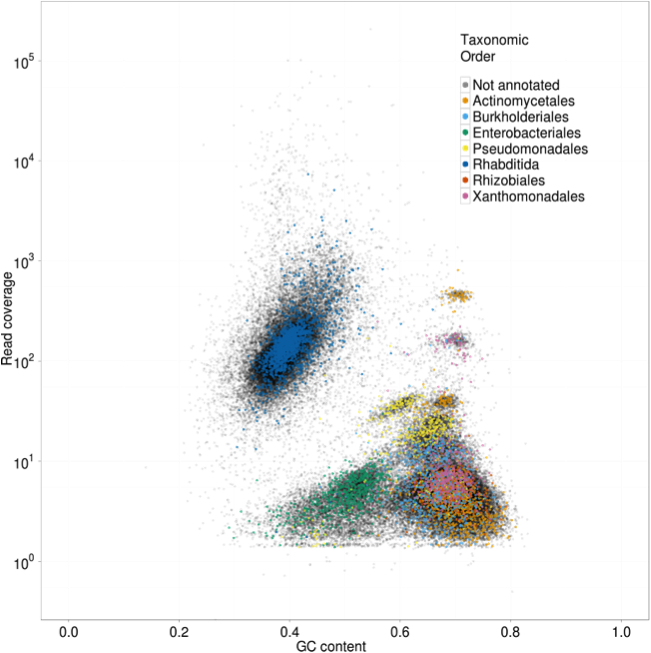
\includegraphics[height=0.7\textheight]{images/blobology}
  \end{center}
\end{frame}

%
\begin{frame}
  \frametitle{Nucleotide $k$-mers}
  Sequence data is necessary to determine $k$-mers/frequencies \\
  \textit{Not possible by experiment}
  \begin{itemize}
    \item \textcolor{hutton_green}{Nucleotides, $k=1$, 4x1-mers} \\
      \url{A, C, G, T}
    \item \textcolor{hutton_blue}{Dinucleotides, $k=2$, 16x2-mers} \\
      \url{AA, AC, AG, AT, CA, CC, CG, CT, GA, GC, GG, GT, TA, TC, TG, TT}
    \item \textcolor{RawSienna}{Triucleotides, $k=1$, 64x3-mers}
    \item \textcolor{hutton_purple}{$k$-nucleotides, $4^k$x$k$-mers}
  \end{itemize}  
\end{frame}

%
\begin{frame}
  \frametitle{$k$-mer spectra
  \footnote{\tiny{\href{http://dx.doi.org/10.1186/gb-2009-10-10-r108
}{Chor \textit{et al.} (2009) \textit{Genome Biol.} doi:10.1186/gb-2009-10-10-r108
}}}
  }
  \textcolor{RawSienna}{$k$-mer spectrum: frequency distribution of observed $k$-mer counts.} \\
  Most species have a unimodal $k$-mer spectrum ($k\approx9$)
  \begin{center}
    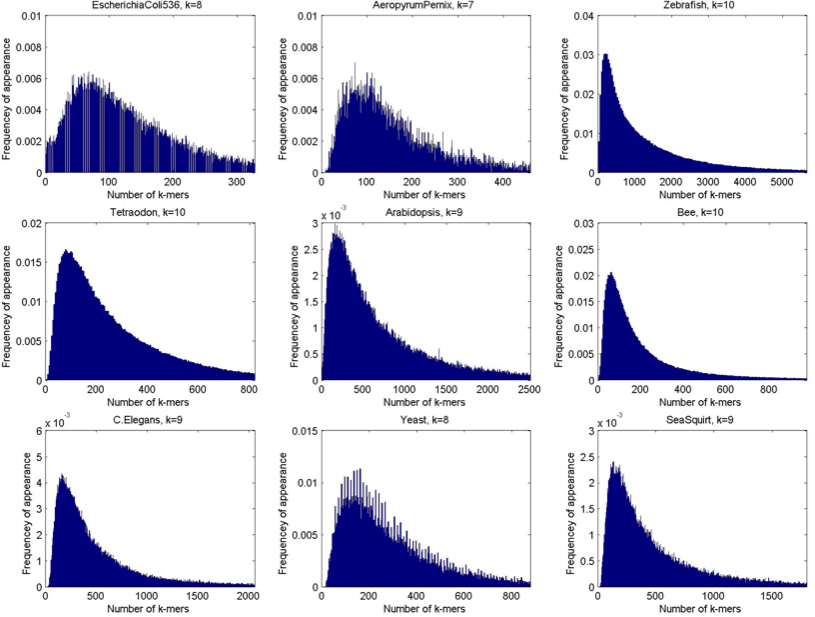
\includegraphics[height=0.6\textheight]{images/kmer_spectra} \\
  \end{center}  
\end{frame}

%
\begin{frame}
  \frametitle{$k$-mer spectra
  \footnote{\tiny{\href{http://dx.doi.org/10.1186/gb-2009-10-10-r108
}{Chor \textit{et al.} (2009) \textit{Genome Biol.} doi:10.1186/gb-2009-10-10-r108
}}}
  }
  \textcolor{RawSienna}{All mammals tested (and some other species) have \textit{multimodal $k$-mer spectra}} \\
  Genomic regions also differ in this property
  \begin{center}
    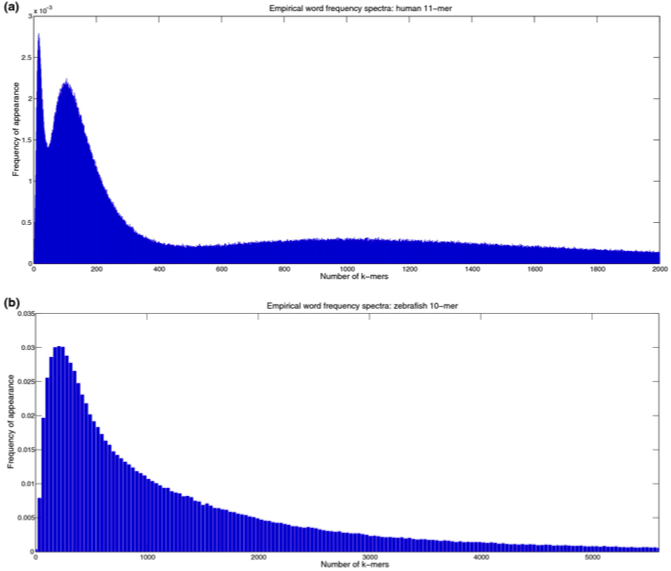
\includegraphics[height=0.4\textheight]{images/kmer_mammal1}
    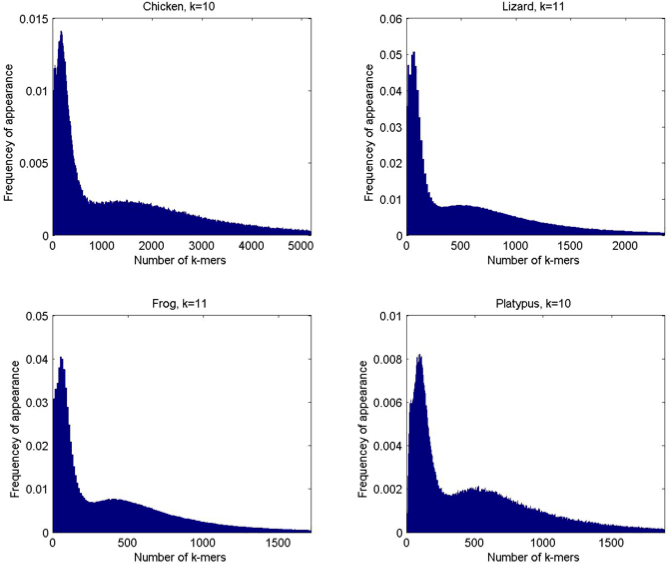
\includegraphics[height=0.4\textheight]{images/kmer_mammal2}    
  \end{center}  
\end{frame}
